\subsection{m5 family}
The first experiment was conducted on the m5 dedicated host. At each throughput level, we executed 
the sockperf command 30 times and averaged the metrics recorded. We extracted the average latency
as well as the 90th and 99.9th percentile values. 
Figure \ref{fig::latencym5} shows the results of the experiment. 
\begin{figure}[H]
\centering
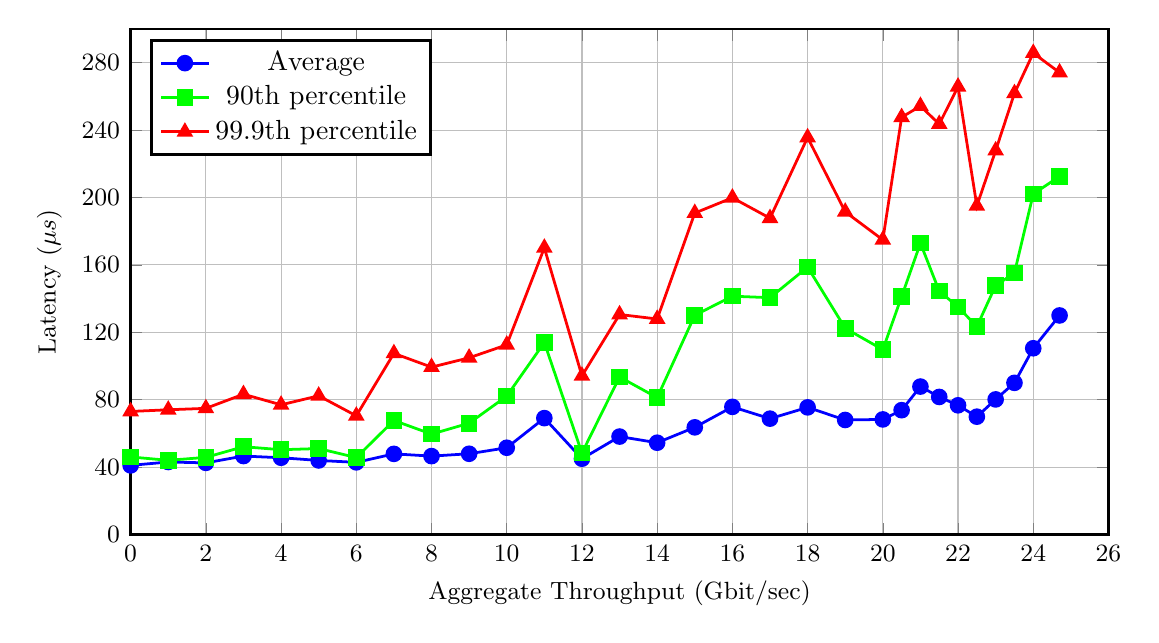
\begin{tikzpicture}
\begin{axis}[
    width=14cm,
    height=8cm,
    xlabel={Aggregate Throughput (Gbit/sec)},
    ylabel={Latency (\(\mu s\))},
    grid=major,
    xmin=0, xmax=26,
    ymin=0, ymax=300,
    xtick={0,2,...,25.5},
    ytick={0,40,80,...,300},
    line width=1pt,
    mark size=2.5pt,
    tick label style={font=\small},
    label style={font=\small},
    legend style={at={(0.02,0.98)},anchor=north west},
    title style={font=\bfseries\small},
]
\addplot[
    mark=*,
    color=blue,
] coordinates {
(0, 41)
(1, 43)
(2, 42.484)
(3, 46.525)
(4, 45.526)
(5, 43.926)
(6, 42.783)
(7, 47.828)
(8, 46.493)
(9, 47.892)
(10, 51.454)
(11, 69.042)
(12, 44.942)
(13, 58.097)
(14, 54.435)
(15, 63.578)
(16, 75.729)
(17, 68.724)
(18, 75.424)
(19, 67.945)
(20, 68.269)
(20.5, 73.756)
(21, 87.778)
(21.5, 81.605)
(22, 76.654)
(22.5, 69.899)
(23, 80.156)
(23.5, 89.978)
(24, 110.510)
(24.7, 129.992)
};
\addlegendentry{Average}

% 90th percentile (2nd value)
\addplot[
    mark=square*,
    color=green,
] coordinates {
(0, 46)
(1, 44)
(2, 45.745)
(3, 52.078)
(4, 50.296)
(5, 50.974)
(6, 45.630)
(7, 67.651)
(8, 59.554)
(9, 66.028)
(10, 82.090)
(11, 113.933)
(12, 48.304)
(13, 93.470)
(14, 81.212)
(15, 130.075)
(16, 141.434)
(17, 140.527)
(18, 158.698)
(19, 122.399)
(20, 109.679)
(20.5, 141.194)
(21, 172.899)
(21.5, 144.428)
(22, 135.069)
(22.5, 123.395)
(23, 147.747)
(23.5, 155.251)
(24, 202.095)
(24.7, 212.558)
};
\addlegendentry{90th percentile}

% 99.9th percentile (3rd value)
\addplot[
    mark=triangle*,
    color=red,
] coordinates {
(0, 73)
(1, 74)
(2, 74.844)
(3, 83.237)
(4, 76.947)
(5, 82.303)
(6, 70.414)
(7, 107.474)
(8, 99.315)
(9, 104.859)
(10, 112.546)
(11, 170.118)
(12, 94.143)
(13, 130.557)
(14, 127.888)
(15, 190.757)
(16, 199.854)
(17, 187.725)
(18, 235.632)
(19, 191.516)
(20, 174.864)
(20.5, 247.645)
(21, 254.280)
(21.5, 243.589)
(22, 265.750)
(22.5, 195.045)
(23, 227.853)
(23.5, 261.827)
(24, 285.742)
(24.7, 274.180)
};
\addlegendentry{99.9th percentile}
\end{axis}
\end{tikzpicture}
\caption{Average Latency vs Bandwidth}
\label{fig::latencym5}
\end{figure}
\noindent
The baseline average latency between the test client and the server was 41 \(\mu s\), which is 
relatively low considering that both reside in the same \ac{AZ}. 
From the start of the experiment up to an aggregate throughput of 9 Gbit/s, latency exhibited 
only minor degradation, increasing by 11.9\% to 47 \(\mu s\).
Beyond this point, latency began to rise significantly in a gradual manner that became sharper,
as the aggregate throughput approached the maximum aggregate throughput of 24.7 Gbit/s. 
It increased from 51 \(\mu s\) at 10 Gbit/s to 130 \(\mu s\) at 24.7 Gbit/s , corresponding to an 155\%
increase. Overall, the experiment revealed a total latency degradation of approximately 217\%, 
a substantial value that could have severe implications for latency-sensitive workloads. \\ 
Furthermore, the results also indicate siginificant variability. 
The 90th percentile latency values were, on average, 41 \(\mu s\) higher than the 
mean, while the 99.9th-percentile values exceeded the mean by 100  \(\mu s\), on average. 
This variability became more pronounced as the mean latency degraded. Figure \ref{fig:sub} illustrates 
the difference between the mean and the 90th-percentile latency value, clearly highlighting 
the increased variability with increased aggregate throughput. 

\begin{figure}[H]
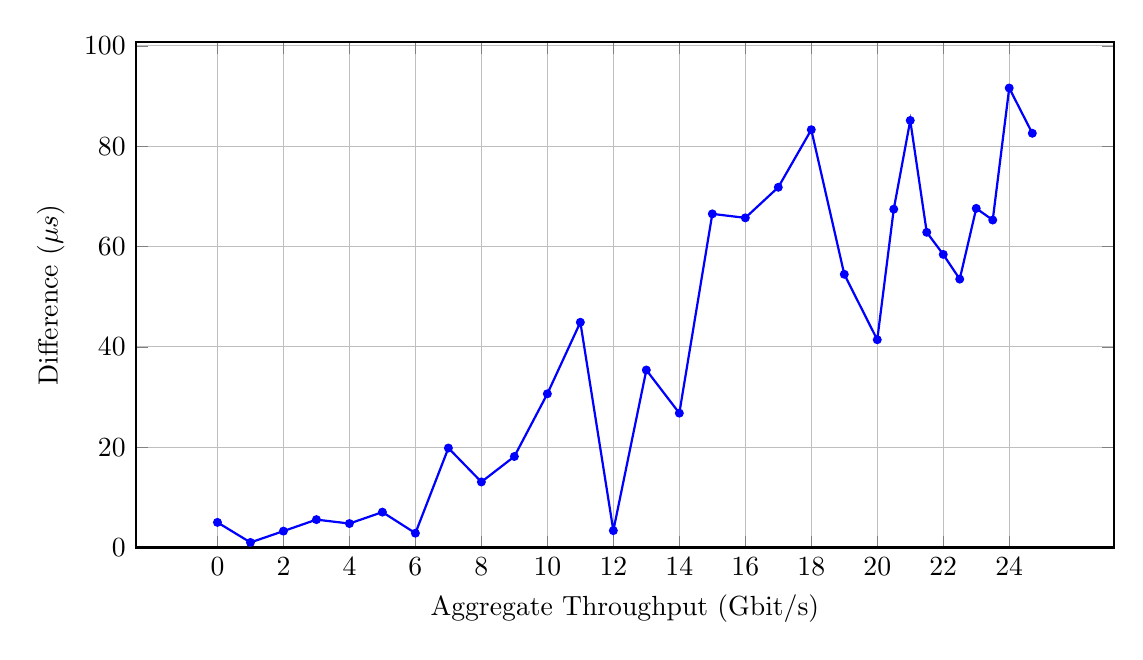
\begin{tikzpicture}
\begin{axis}[
    width=14cm,
    height=8cm,
    grid=major,
    xlabel={Aggregate Throughput (Gbit/s)},
    ylabel={Difference (\(\mu s\))},
    ymin=0,
    xtick={0,2,4,6,8,10,12,14,16,18,20,22,24},
    ytick distance=20,
    thick,
    legend style={at={(0.98,0.02)},anchor=south east}
]

\addplot[
    blue,
    mark=*,
    mark options={scale=0.6},
] coordinates {
(0, 5.000)
(1, 1.000)
(2, 3.261)
(3, 5.553)
(4, 4.770)
(5, 7.048)
(6, 2.847)
(7, 19.823)
(8, 13.061)
(9, 18.136)
(10, 30.636)
(11, 44.891)
(12, 3.362)
(13, 35.373)
(14, 26.777)
(15, 66.497)
(16, 65.705)
(17, 71.803)
(18, 83.274)
(19, 54.454)
(20, 41.410)
(20.5, 67.438)
(21, 85.121)
(21.5, 62.823)
(22, 58.415)
(22.5, 53.496)
(23, 67.591)
(23.5, 65.273)
(24, 91.585)
(24.7, 82.566)
};
\end{axis}
\end{tikzpicture}
\caption{Difference between the 90th-percentile latency values and the mean}
\label{fig:sub}
\end{figure}
